\chapter{Населённые пункты}
\label{ch:human-settlement}

	В главе исследуется объект Викиданных \wdqName{населённый пункт}{486972} и его свойства. В каждом из разделов представлены задачи, решённые с помощью SPARQL-запросов. 

%%%%%%%%%%%%%%%% Упражнение 1 %%%%%%%%%%%%%%%% 
\marginnote{ У какого населённого пункта России самая низкая плотность населения?
\begin{itemize}
\item \href{https://w.wiki/4dNt}{Алейск} в \href{https://w.wiki/3vZQ}{Алтайском крае}
\item \href{https://w.wiki/4dNu}{Заречный} в \href{https://w.wiki/4dNy}{Свердловской области}
\item \href{https://w.wiki/4dNv}{Барабинск} в \href{https://w.wiki/4dP3}{Новосибирской области}
\item \href{https://w.wiki/4dNw}{Зверево} в \href{https://w.wiki/4dP4}{Ростовской области}
\end{itemize}
См. ответ~\ref{answer:human_settlements_density} на с.~\pageref{answer:human_settlements_density}.}

Был получен список населённых пунктов, построен список стран по суммарному количеству населения. Построили пузырьковые диаграммы по суммарному количеству населения,
проживающего в объектах типа «населённый пункт».

Построена диаграмма, показывающая долю населения страны, проживающего в населённых пунктах. Диаграмма показывает, что высокий процент населения, проживающего в населённых пунктах, приходится на менее промышленные страны, в то время как в более индустриальных странах меньшая доля населения проживает в населённых пунктах. 

%%%%%%%%%%%%%%%% Упражнение 2 %%%%%%%%%%%%%%%%
\marginnote{ Выберите, представленный герб относится к населённым пунктам Российской Федерации или нет, изображенный на рис. \ref{fig:flag_question_human_settlements1}? }
\begin{marginfigure}[0.0cm] {
\setlength{\fboxsep}{0pt}%
\setlength{\fboxrule}{1pt}%
\fcolorbox{gray}{gray}{
\includegraphics[width=0.5\linewidth]{./chapter/human_settlement/Aznakeevskii_rayon_gerb.png}}%
}
  \caption{Герб населённого пункта.}%
  \label{fig:flag_question_human_settlements1}%
\end{marginfigure}

\marginnote{
См. ответ~\ref{answer:flag_human_settlements} на с.~\pageref{answer:flag_human_settlements}.
}

На 2017 год Википедия описывает примерно половину населённых пунктов (75 тыс.), Викиданные содержат менее 3\% таких поселений (4 тыс.) относительно данных переписи за 2010 год (155,5 тыс.). На 2021 год Викиданные содержат менее 12\% таких поселений (17 тыс.) относительно данных переписи за 2010 год (155,5 тыс.). 

Построили диаграммы количества ученых по родам деятельности родившихся в сельских и городских полесениях.

Для улучшения результатов решения вышеописанных задач находили более общие классы и указывали их в исследуемом объекте с помощью свойства экземпляры. Трудность исследования вызвана отсутствием чёткой типологии населённых пунктов (например, от численности населения) в законодательстве России и в Викиданных.

%%%%%%%
\section{Список <<Населённых пунктов>>}

Для построения списка всех населённых пунктов нам потребуются объект \wdqName{населённый пункт}{486972} и свойство \wdProperty{31}{экземпляр} (листинг ~\protect\ref{lst:human-settlement1}).

\begin{lstlisting}[ language=SPARQL, 
                    caption={\href{https://w.wiki/4d7x}{Список всех населённых пунктов}\protect\footnotemark},
                    label=lst:human-settlement1,
                    texcl 
                    ]
# List of all human settlements
SELECT ?hum ?humLabel WHERE{
  ?hum wdt:P31 wd:Q486972. # instance of human settlement
  SERVICE wikibase:label{bd:serviceParam wikibase:language "ru,en"}
}
\end{lstlisting}%
\footnotetext{Получен \num{411393} записи в 2017 году.  Ссылка на SPARQL-запрос: \href{https://w.wiki/4d7x}{https://w.wiki/4d7x}}

В 2021 году оказалось не возможно получить список населённых пунктов из-за большого числа объектов и поэтому слишком долгой работы (листинг ~\protect\ref{lst:human-settlement1}). Для получения результата произведём подсчёт всех населённых пунктов с помощью функции \textit{COUNT()} (листинг ~\protect\ref{lst:human-settlement2}).

\index{SPARQL!COUNT!Количество всех населённых пунктов}
\begin{lstlisting}[ language=SPARQL, 
                    caption={\href{https://w.wiki/4d7s}{Количество всех населённых пунктов}\protect\footnotemark},
                    label=lst:human-settlement2,
                    texcl 
                    ]
# Number of human settlements
SELECT (COUNT(?hum) AS ?count) WHERE {
  ?hum wdt:P31 wd:Q486972. # instance of human settlement  
}
\end{lstlisting}%
\footnotetext{Получили \num{563126} населённых пунктов в 2021 году. Ссылка на SPARQL-запрос: \href{https://w.wiki/4d7s}{https://w.wiki/4d7s}}

Почти пустыми и малоинформативными оказались такие населёнными пункты: \wdqName{Zangabad}{146827} (2 свойства) и \wdqName{Zapallar}{147201} (2 свойства). Среди отечественных населённых пунктов: \wdqName{Borisovo}{4093951} (3 свойства) и \wdqName{Zakhod}{18777794} (3 свойства).

Среди населённых пунктов принадлежащих России в Викиданных больше всего свойств по данным ProWD у \href{http://www.wikidata.org/entity/Q128499}{Ялты} (36 свойств). Лидером по всему миру является \href{http://www.wikidata.org/entity/Q1490}{Токио} (73 свойства)\autocite{humansettlements_ProWD}.

%%%%%%%
\section{Список стран по суммарному количеству населения}

Построим упорядоченный список стран по суммарному количеству населения, проживающего в <<населённых пунктах>> (листинг ~\protect\ref{lst:human-settlement3}).

\index{SPARQL!SUM!Список стран по суммарному количеству населения, проживающего в <<населённых пунктах>>}
\index{SPARQL!GROUP BY!Список стран по суммарному количеству населения, проживающего в <<населённых пунктах>>}
\lstset{numbers=left, firstnumber=1, frame=single}
\begin{lstlisting}[ language=SPARQL, 
                    caption={\href{https://w.wiki/4d9M}{Список стран по суммарному количеству населения, проживающего в <<населённых пунктах>>}\protect\footnotemark},
                    label=lst:human-settlement3,
                    texcl 
                    ]
# List of countries by population in settlements
SELECT ?country ?countryLabel (SUM(?population) as ?sumPopulation)
WHERE {
  ?hum wdt:P31 wd:Q486972;  	# instance of human settlement
       wdt:P17 ?country;    	# in the ?country
       wdt:P1082 ?population. # has ?population
  SERVICE wikibase:label{bd:serviceParam wikibase:language "ru,en"}
}
GROUP BY ?country ?countryLabel 
ORDER BY DESC (?sumPopulation)
\end{lstlisting}%
\footnotetext{Получена \num{161} страна в 2017 году и \num{213} стран в 2021 году. Ссылка на SPARQL-запрос: \href{https://w.wiki/4d9M}{https://w.wiki/4d9M}}

Для подсчета насления по странам, используем команду \textit{SUM()} на второй строке скрипта (листинг ~\protect\ref{lst:human-settlement3}). Для группировки населённых пунктов по странам, используем команду \textit{GROUP BY} на девятой строке скрипта (листинг ~\protect\ref{lst:human-settlement3}).

Пузырьковая диаграмма на рис. ~\ref{fig:human-settlement-1} показывает соотношение стран по количеству населения в <<населённых пунктах>> в 2017 году.

\begin{figure}
\centering
	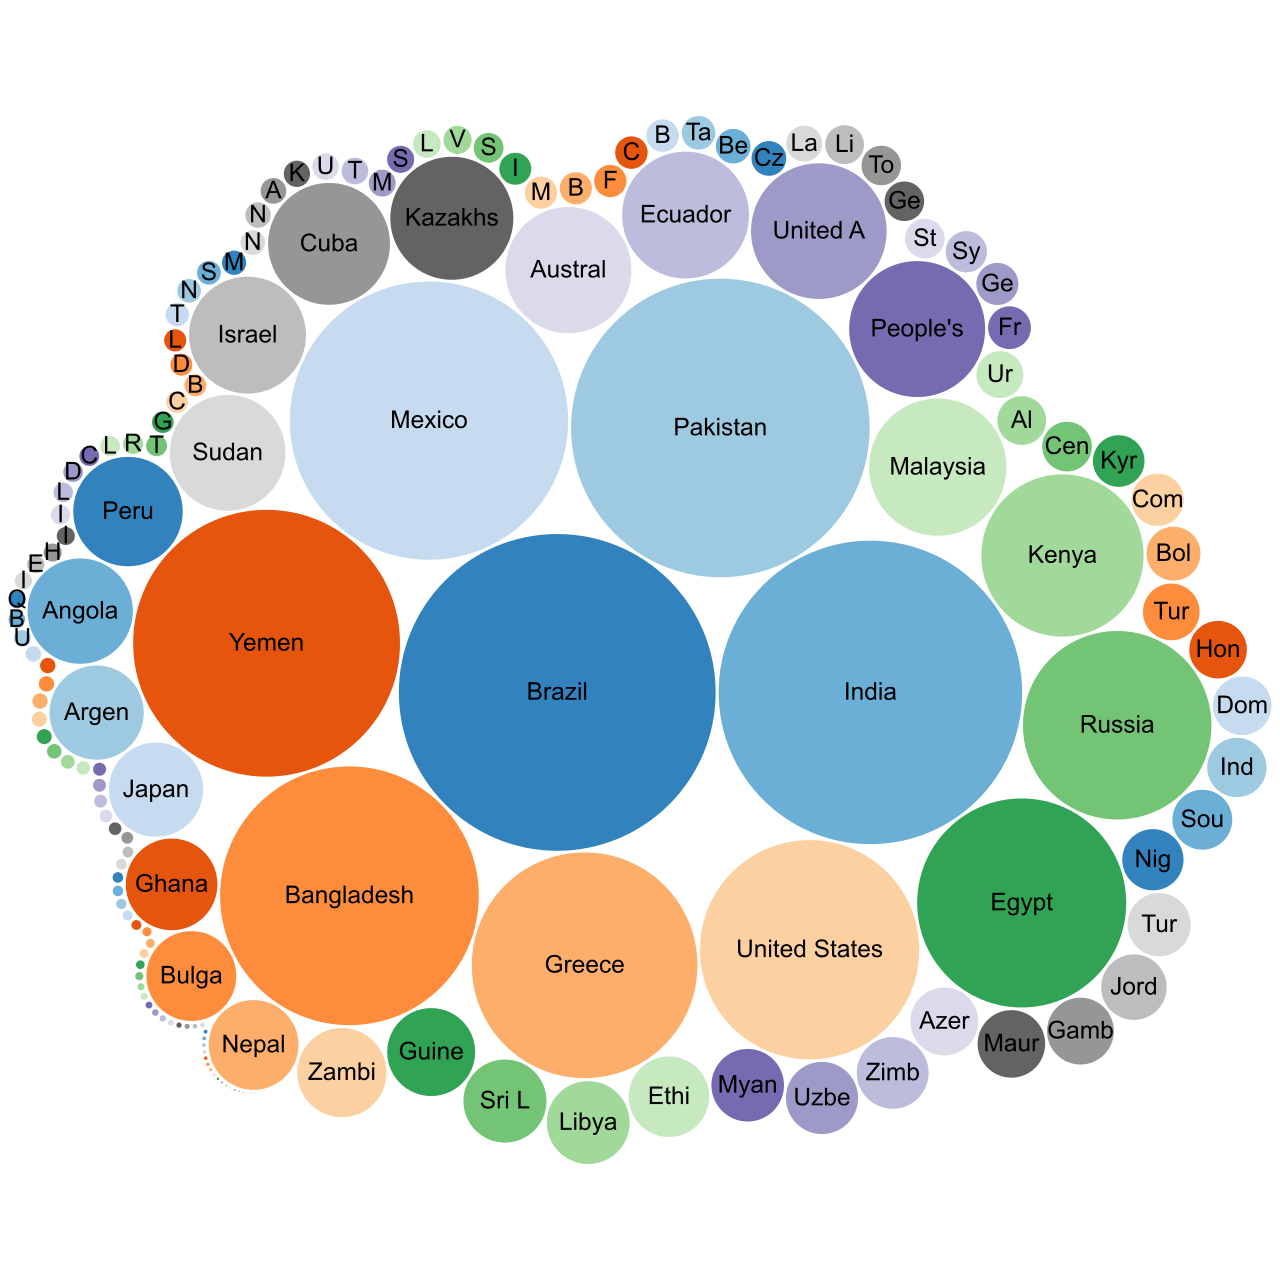
\includegraphics[width=0.9\linewidth]{./chapter/human_settlement/AnnaBubbleHumanSettlement.jpg}
	\label{fig:human-settlement-1}
    \caption[Пузырьковая диаграмма  по суммарному количеству населения в населённых пунктах, 2017.]{Пузырьковая диаграмма  по суммарному количеству населения, проживающего в <<населённых пунктах>> на 2017 год. Размер пузырька соответствует количеству населения, проживающего в <<населённых пунктах>> одной страны. Ссылка на SPARQL-запрос: \href{https://w.wiki/4dAv}{https://w.wiki/4dAv}}
\end{figure}

\begin{figure}
\centering
	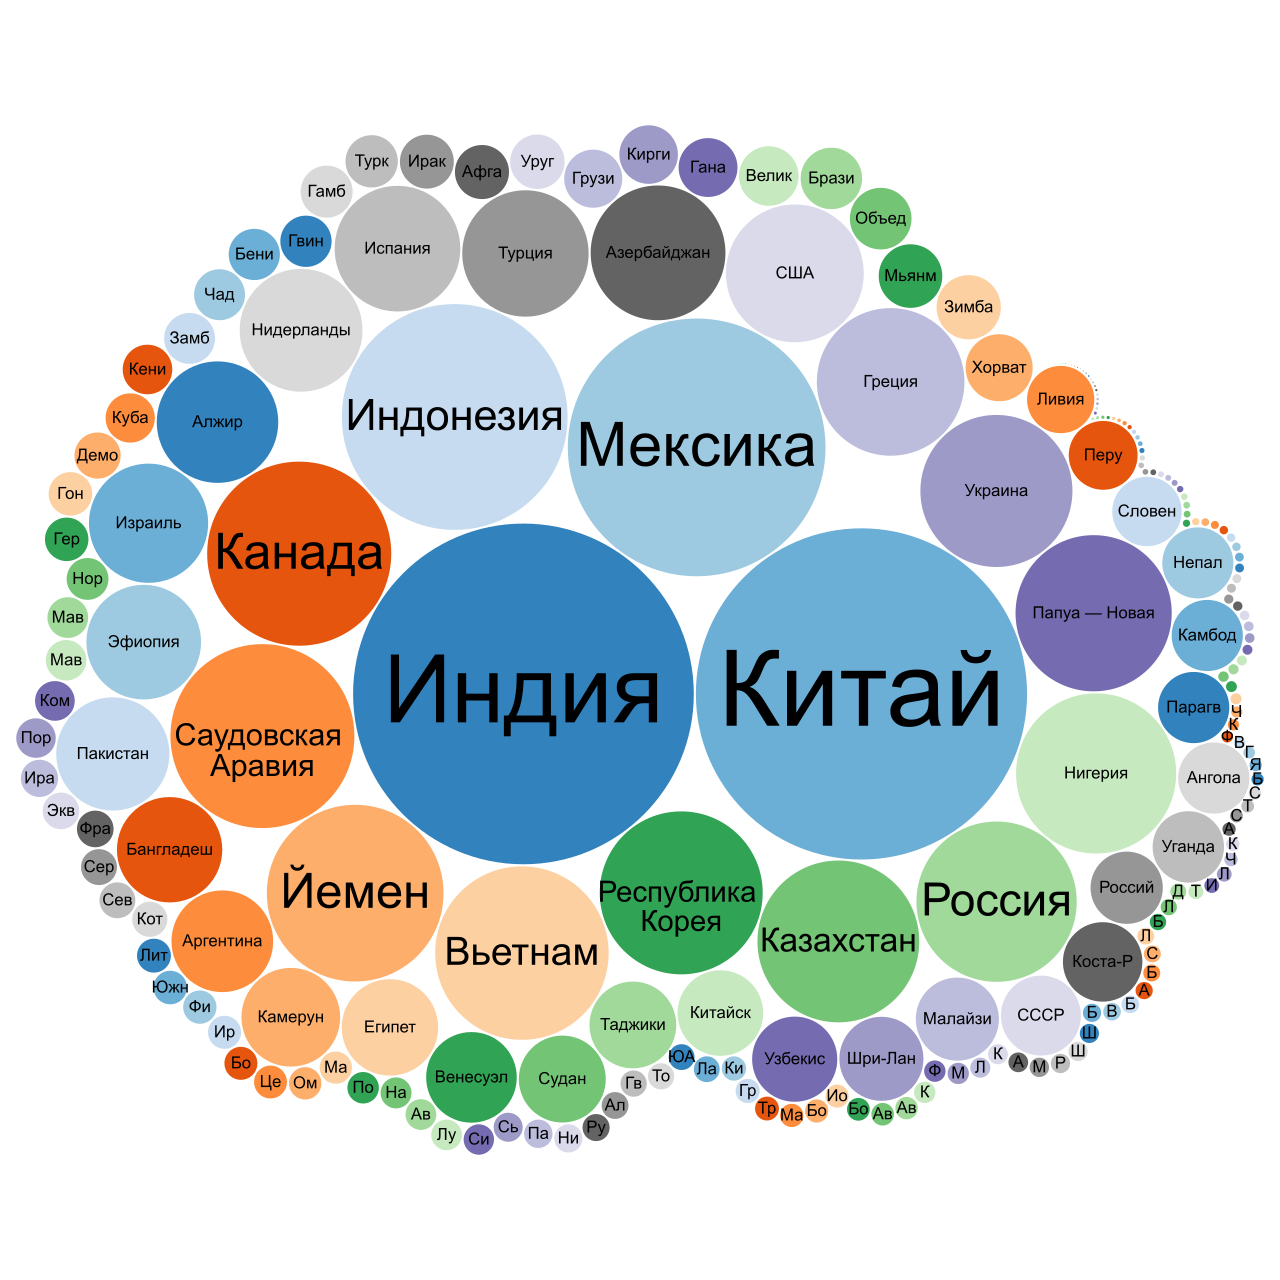
\includegraphics[width=0.9\linewidth]{./chapter/human_settlement/LeonidBubbleHumanSettlement.jpg}
	\label{fig:human-settlement-2}
	\caption[Пузырьковая диаграмма  по суммарному количеству населения в населённых пунктах, 2021.]{Пузырьковая диаграмма  по суммарному количеству населения, проживающего в <<населённых пунктах>> на 2021 год. Размер пузырька соответствует количеству населения, проживающего в <<населённых пунктах>> одной страны. Ссылка на SPARQL-запрос: \href{https://w.wiki/4dAv}{https://w.wiki/4dAv}}
\end{figure}

В 2017 году больше всего количество населения проживало в объектах <<населённый пункт>> в таких странах, как: \href{http://www.wikidata.org/entity/Q155}{Бразилия} (\num{12} млн), \href{http://www.wikidata.org/entity/Q843}{Пакистан} (\num{10} млн), \href{http://www.wikidata.org/entity/Q96}{Мексика} (\num{8} млн), \href{http://www.wikidata.org/entity/Q805}{Йемен} (\num{8} млн), \href{http://www.wikidata.org/entity/Q668}{Индия} (\num{7} млн), \href{http://www.wikidata.org/entity/Q902}{Бангладеш} (\num{7} млн). 

На рис. ~\ref{fig:human-settlement-2} можно увидеть список стран на 2021 год: \href{http://www.wikidata.org/entity/Q668}{Индия} (\num{30} млн), \href{http://www.wikidata.org/entity/Q148}{Китай} (\num{28} млн), \href{http://www.wikidata.org/entity/Q96}{Мексика} (\num{17} млн), \href{http://www.wikidata.org/entity/Q252}{Индонезия} (\num{13} млн), \href{http://www.wikidata.org/entity/Q16}{Канада} (\num{9} млн), \href{http://www.wikidata.org/entity/Q851}{Саудовская Аравия} (\num{9} млн). 

Итоги запросов в 2017 и 2021 имеют сильно разные результаты. За четыре года в Индии прибавилось 23 млн человек, из этого можно сделать вывод, что за четыре года информация в Викиданных стала более полной по населённым пунктам.

%%%%%%%%%%%

\subsection{Расширение понятия <<населённый пункт>>}

%%%%%%%%%%%%%%%% Упражнение 2 %%%%%%%%%%%%%%%%
\marginnote{
Выберите, представленный герб относится к населённым пунктам Российской Федерации или нет, изображенный на рис. \ref{fig:flag_question_human_settlements2}?
}
\begin{marginfigure}[0.0cm]
{
\setlength{\fboxsep}{0pt}%
\setlength{\fboxrule}{1pt}%
\fcolorbox{gray}{gray}{
\includegraphics[width=0.5\linewidth]{./chapter/human_settlement/Coat_of_Arms_of_Asbest_(Sverdlovsk_oblast).png}}%
}
  \caption{Герб населённого пункта.}%
  \label{fig:flag_question_human_settlements2}%
\end{marginfigure}

\marginnote{
См. ответ~\ref{answer:flag_human_settlements} на с.~\pageref{answer:flag_human_settlements}.
}

Далее классом будем называть каждое свойство \wdProperty{31}{экземпляра} в исследуемом объекте на Викиданных. Попробуем получить более полный результат стрипта (листинг ~\protect\ref{lst:human-settlement3}). Для это нужно изучить класс \wdqName{населенный пункт}{486972} из свойства экземпляр. Рассмотрим город \wdqName{Петрозаводск}{1895} он имеет четыре класса (\wdqName{административно-территориальная единица России}{192287}; \wdqName{город с населением более \num{100000} человек}{1549591}; \wdqName{населённый пункт}{486972}; \wdqName{город}{7930989}). Три из этих классов являются схожими по значению и используются совместно с интересующим нас классом <<населённый пункт>>. Выведем список классов поселений и их количество для объектов имеющих свойство \wdProperty{1082}{численность населения} и принадлежащие стране \wdqName{России}{159} (листинг ~\protect\ref{lst:human-settlement4}). 

\index{SPARQL!COUNT!Список классов поселений и их количество для объектов имеющих свойство <<численность населения>> в России}
\begin{lstlisting}[ language=SPARQL, 
                    caption={\href{https://w.wiki/4dBU}{Список классов поселений и их количество для объектов имеющих свойство <<численность населения>> в России}\protect\footnotemark},
                    label=lst:human-settlement4,
                    texcl 
                    ]
# List of settlement classes and their number for objects with 
# the property "population" in Russia
SELECT ?class ?classLabel (COUNT(?class) AS ?count) WHERE {
  {
  SELECT ?class ?classLabel ?humLabel WHERE {
   ?hum wdt:P17 wd:Q159;  # settlement in the Russia
        wdt:P1082 ?population; # has ?population
        wdt:P31 ?class. # has ?class
    SERVICE wikibase:label{bd:serviceParam wikibase:language "ru,en"}
   }
  }
}
GROUP BY ?class ?classLabel
ORDER BY DESC (?count)
\end{lstlisting}%
\footnotetext{Получили 216 разных классов поселений. Ссылка на SPARQL-запрос: \href{https://w.wiki/4dBU}{https://w.wiki/4dBU}}

Класс <<населённый пункт>> оказался на десятом месте и набрал всего \num{1122} упоминаний. Результаты скрипта (листинг ~\protect\ref{lst:human-settlement4}) представлены в таблице ~\ref{tab:human-settlement1}.

\begin{table}[h]
\caption{Таблица классов и их количество упоминаний среди объектов имеющих свойство <<численность населения>> в России}
\begin{tabular}{|l|l|l|}
\hline
номер & название класса                       						& количество упоминаний	\\ \hline
1         & \wdqName{сельское поселение в России}{634099}     			& \num{18104}                		\\
2         & \wdqName{деревня}{5084}              						& \num{14795}                		\\
3         & \wdqName{село}{532}								& \num{9875}               		\\ 
4         & \wdqName{посёлок}{2514025}						& \num{4418}               		\\ 
7         & \wdqName{хутор}{2023000}							& \num{1733}               		\\ 
9         & \wdqName{город}{7930989}							& \num{1172}               		\\ 
10       & \wdqName{населённый пункт}{486972}					& \num{1149}               		\\ 
11       & \wdqName{посёлок городского типа России}{15078955}		& \num{665}               		\\ 
21       & \wdqName{город с населением более 100 000 человек}{1549591}	& \num{108}               		\\ \hline
\end{tabular}
\caption{Таблица классов и их количество упоминаний среди объектов имеющих свойство <<численность населения>> в России}
\label{tab:human-settlement1}
\end{table}

Из результатов (листинг ~\protect\ref{lst:human-settlement4}), видно, что класс <<населённый пункт>> используется совместно не со всеми класами поселений. Попробуем получить еще раз результат для России на основе (листинг ~\protect\ref{lst:human-settlement3}), используя дополнительные классы из таблицы ~\ref{tab:human-settlement1} под номерами: 1, 2, 3, 4, 7 и 11. В дальнейшем комбинация этих классов будет упоминаться, как сельские поселения. Произведём новый подсчёт количества населения <<населённых пунктов>> в России, дополненый сельскими поселениями (листинг ~\protect\ref{lst:human-settlement5}).

\index{SPARQL!SUM!Подсчет количества населения <<населённых пунктов>> и поселения сельского типа}
\begin{lstlisting}[ language=SPARQL, 
                    caption={\href{https://w.wiki/4dBy}{Подсчет количества населения <<населённых пунктов>> и поселения сельского типа}\protect\footnotemark},
                    label=lst:human-settlement5,
                    texcl 
                    ]
# total population in rural settlements in Russia
SELECT (SUM(?population) as ?sumPopulation) 
WHERE{
  VALUES ?type {wd:Q634099 wd:Q5084 wd:Q532 wd:Q2514025 wd:Q2023000 
               wd:Q15078955}
  ?hum wdt:P31 ?type; # instance of human settlement
    wdt:P17 wd:Q159;   # settlement in Russia
    wdt:P1082 ?population. # settlement has ?population
}
ORDER BY DESC (?sumPopulation)
\end{lstlisting}%
\footnotetext{Получили \num{60,5} млн население <<населённых пунктов>> и поселений сельского типа в России. Ссылка на SPARQL-запрос: \href{https://w.wiki/4dBy}{https://w.wiki/4dBy}}

К численности населения в <<населённых пунктах>> (\num{6,5} млн человек) в результатах (листинг ~\protect\ref{lst:human-settlement3}), добавилось еще \num{54} млн человек из поселений сельского типа. Из чего следует, что класс <<населённый пункт>> мало заполнен на Викиданных. Возможно в будующем все поменяется и класс <<населённый пункт>> будет наполняться. 


%%%%%
\subsection{Полнота Викиданных}

Населённый пункт — это общее название мест с постоянными жителями\autocite{Humansettlements_Dictionary}. По версии редакторов Викиданных в понятие насёленный пункт входят города, сёла, деревни и другие\footnote{Полный список можно увидеть в разделе <<Cписок классов, сопутствующих <<населённому пункту>> в свойстве <<экземпляр>>>> на с.~\pageref{human-settlement:tag1}.}.
Точной информации о количестве населённых пунктов в мире не было найдено. Поэтому проверим полноту населённых пунктов, которые есть в Викиданных и которые использовались для решения задачи. В задачах выше мы использовали свойста \wdProperty{1082}{численность населения} и \wdProperty{17}{государство} (привязанность к стране). Исходя из этого проверку полноты разделим на подзадачи: 
\begin{enumerate} 
  \item Проверка заполнености свойства <<численность населения>>.
  \item Проверка принадлежности к <<государству>>.
\end{enumerate}

%%%%%
\subsection{Проверка заполнености свойства <<численность населения>> }

Для этого напишем \href{https://w.wiki/4FUz}{SPARQL-запрос}\footnotemark, который выведет населённые пункты с незаполненным свойством \href{http://www.wikidata.org/entity/P1082}{численность населения}. 
\footnotetext{ В 2017 году запрос выдал \num{372997} населённых пунктов с незаполненным свойством <<численность населения>>. Проводя ту же проверку в 2021 году, запрос выдал \num{507078} таких населённых пунктов. Ссылка на SPARQL-запрос: \href{https://w.wiki/4FUz}{https://w.wiki/4FUz}} 
Произведя расчеты получаем, что только у 9,3\% населенных пунктов мира указано свойство <<численность населения>> на 2017 год. В 2021 получаем 11,2\% населенных пунктов мира с заполненным свойство <<численность населения>>.

%%%%%
\subsection{Проверка принадлежности к <<государству>>}

А теперь посмотрим населённые пункты, у которых не указана принадлежность к какой-либо стране~--- \href{https://w.wiki/4FV8}{SPARQL-запрос}\footnotemark.

\footnotetext{В 2017 году нашлось \num{8427} объектов, у которых не указана принадлежность к какой-либо стране. В 2021 году таких объектов уже больше~--- \num{27824}. Ссылка на SPARQL-запрос: \href{https://w.wiki/4FV8}{https://w.wiki/4FV8}}
Получалется неполная картина при получении результата решения данной задачи о суммарном количестве населения в населённых пунктах по странам из-за того, что такие объекты существуют.

%%%%%
\section{Доля населения страны, проживающего в <<населённых пунктах>>}

Построим упорядоченный список стран доли населения (в процентах), проживающего в \href{http://www.wikidata.org/entity/Q486972}{населённых пунктах}, относительно числа всех жителей страны (листинг ~\protect\ref{lst:human-settlement6}).

%%%%%%%%%%%%%%%% Упражнение 2 %%%%%%%%%%%%%%%%
\marginnote{
Выберите, представленный герб относится к населённым пунктам Российской Федерации или нет, изображенный на рис. \ref{fig:flag_question_human_settlements3}?
}
\begin{marginfigure}[0.0cm]
{
\setlength{\fboxsep}{0pt}%
\setlength{\fboxrule}{1pt}%
\fcolorbox{gray}{gray}{
\includegraphics[width=0.5\linewidth]{./chapter/human_settlement/Loučovice_CoA.jpg}}%
}
  \caption{Герб населённого пункта.}%
  \label{fig:flag_question_human_settlements3}%
\end{marginfigure}

\marginnote{
См. ответ~\ref{answer:flag_human_settlements} на с.~\pageref{answer:flag_human_settlements}.
}

\index{SPARQL!SUM!Соотношение количества людей, проживающих в населённых пунктах, к количеству всех людей в стране}
\begin{lstlisting}[ language=SPARQL, 
                    caption={\href{https://w.wiki/4dE3}{Соотношение количества людей, проживающих в населённых пунктах, к количеству всех людей в стране}\protect\footnotemark},
                    label=lst:human-settlement6,
                    texcl 
                    ]
# An ordered list of the ratio of the number of people living in 
# "human\_settlement" to the number of inhabitants in the country.
SELECT ?country ?countryLabel ?proportionPopulation WHERE {
 SELECT ?country ?countryLabel (SUM(?population / ?pop) 
        as ?proportionPopulation) WHERE {
  ?hum wdt:P31 wd:Q486972;    # instances of human settlement  
       wdt:P17 ?country;         # has ?country 
       wdt:P1082 ?population.    # has ?population
  ?country wdt:P1082 ?pop.    # population in the country
  SERVICE wikibase:label{bd:serviceParam wikibase:language "ru,en"}
 }
 GROUP BY ?country ?countryLabel
}
ORDER BY ?proportionPopulation
\end{lstlisting}%
\footnotetext{Получено \num{158} результатов в 2017 году и \num{206} результатов в 2021 году. Ссылка на SPARQL-запрос: \href{https://w.wiki/4dE3}{https://w.wiki/4dE3}}

Столбчатая диаграмма на рис. ~\ref{fig:human-settlement-3} позволяет увидеть для каждой отдельной страны отношение количества людей, проживающих в \href{http://www.wikidata.org/entity/Q486972}{населённых пунктах}, к числу жителей в стране на 2017 год.

\begin{figure*}
    \setlength{\fboxsep}{0pt}%
    \setlength{\fboxrule}{1pt}%
    \fcolorbox{gray}{gray}{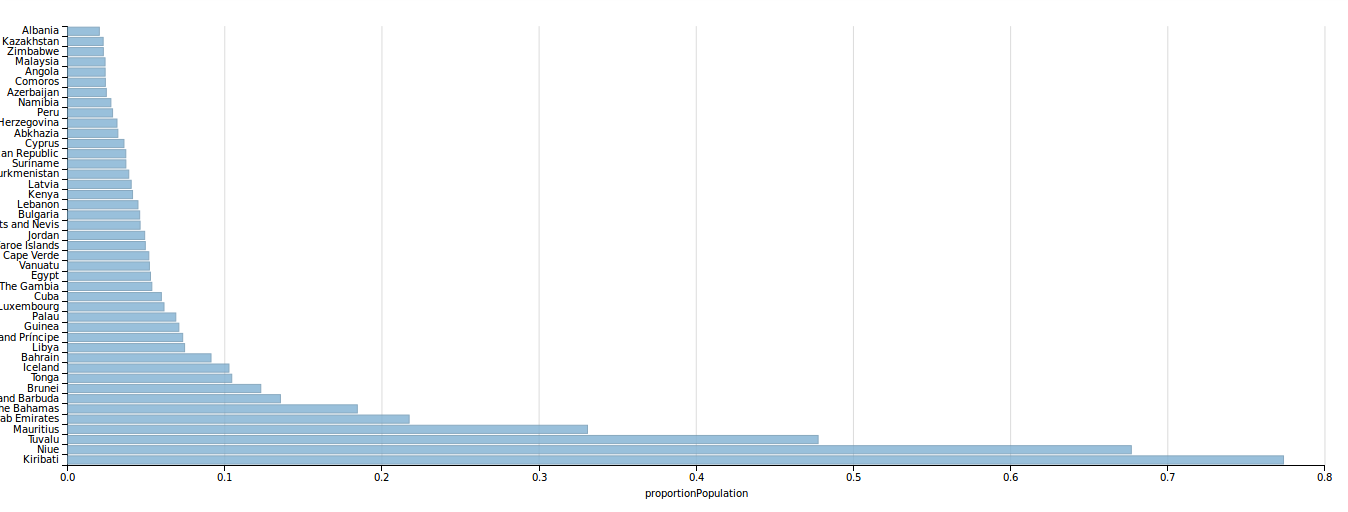
\includegraphics[width=1\linewidth]{./chapter/human_settlement/AnnaShareHumanSettlement.png}}
	\label{fig:human-settlement-3}
	\caption[Диаграмма доли населения страны, 2017.]{Диаграмма доли населения страны, проживающего в <<населённых пунктах>> на 2017 год. Ссылка на SPARQL-запрос: \href{https://w.wiki/4dE3}{https://w.wiki/4dE3}}%
\end{figure*} 

\begin{figure*}
    \setlength{\fboxsep}{0pt}%
    \setlength{\fboxrule}{1pt}%
    \fcolorbox{gray}{gray}{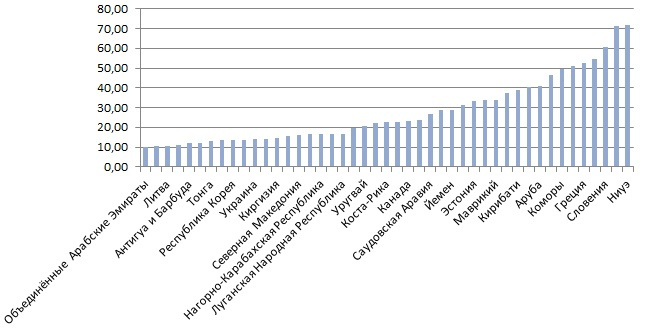
\includegraphics[width=1\linewidth]{./chapter/human_settlement/LeonidShareHumanSettlement.jpg}}
	\label{fig:human-settlement-4}
	\caption[Диаграмма доли населения страны, 2021.]{Диаграмма доли населения страны, проживающего в <<населённых пунктах>> на 2021 год. В 2021 на диаграмму попали только страны с населением более 5 млн человек. Ссылка на SPARQL-запрос: \href{https://w.wiki/4dDx}{https://w.wiki/4dDx}}%
\end{figure*} 

На рис. ~\ref{fig:human-settlement-3} из графика видно, что наиболее высокий процент в 2017 году приходился на следующие страны: Кирибати (78\%), Ниуэ (70\%), Греция (53\%), Тувалу (48\%), Коморы (43\%), Маврикий (42\%). В 2021 году появились изменения : Нигерия (93\%), Папуа — Новая Гвинея (71\%), Израиль (50\%), Греция (47\%), Азербайджан (47\%), Казахстан (37\%). Интересно заметить, что в основном это маленькие островные государства. Вероятно, большая часть жителей этих стран сконцентрирована в населённых пунктах.

На 2017 год рассматривая отдельно страны большой восьмёрки, доля жителей в \href{http://www.wikidata.org/entity/Q486972}{населённых пунктах} составила: \href{http://www.wikidata.org/entity/Q159}{Россия} (\num{2.98}\%), \href{http://www.wikidata.org/entity/Q30}{США} (\num{1.76}\%), \href{http://www.wikidata.org/entity/Q17}{Япония} (\num{0.80}\%), \href{http://www.wikidata.org/entity/Q16}{Канада} (\num{0.26}\%), \href{http://www.wikidata.org/entity/Q142}{Франция} (\num{0.20}\%), \href{http://www.wikidata.org/entity/Q183}{Германия} (\num{0.24}\%), \href{http://www.wikidata.org/entity/Q145}{Великобритания} (\num{0.18}\%), \href{http://www.wikidata.org/entity/Q38}{Италия} (\num{0.07}\%). В 2021 году значения доли населения снизились: \href{http://www.wikidata.org/entity/Q159}{Россия} (0.045\%), \href{http://www.wikidata.org/entity/Q30}{США} (\num{0.014}\%), \href{http://www.wikidata.org/entity/Q17}{Япония} (\num{0.008}\%), \href{http://www.wikidata.org/entity/Q16}{Канада} (\num{0.23}\%), \href{http://www.wikidata.org/entity/Q142}{Франция} (\num{0.005}\%), \href{http://www.wikidata.org/entity/Q183}{Германия} (\num{0.005}\%), \href{http://www.wikidata.org/entity/Q145}{Великобритания} (\num{0.014}\%), \href{http://www.wikidata.org/entity/Q38}{Италия} (\num{0.0005}\%). Отметим, что это страны промышленно развитые.

%%%%%%%%%%%%%%%% Упражнение 2 %%%%%%%%%%%%%%%%
\marginnote{
Выберите, представленный герб относится к населённым пунктам Российской Федерации или нет, изображенный на рис. \ref{fig:flag_question_human_settlements4}?
}
\begin{marginfigure}[0.0cm]
{
\setlength{\fboxsep}{0pt}%
\setlength{\fboxrule}{1pt}%
\fcolorbox{gray}{gray}{
\includegraphics[width=0.5\linewidth]{./chapter/human_settlement/POL_Otynia_COA.png}}%
}
  \caption{Герб населённого пункта.}%
  \label{fig:flag_question_human_settlements4}%
\end{marginfigure}

\marginnote{
См. ответ~\ref{answer:flag_human_settlements} на с.~\pageref{answer:flag_human_settlements}.
}

Построенная диаграмма подтверждает следующую гипотезу: высокий процент населения страны, проживающего в \wdqName{населённых пунктах}{486972}, указывает на более аграрную страну. Исходя из представленных выше диаграмм видно, что наиболее высокий процент населения страны, проживающего в населённых пунктах, приходится на островные, южные, жаркие страны, в которых, по-видимому, менее развита промышленность (маленькая территория, небольшое количество населения, удалённость от материков). А индустриальные страны (большой восьмёрки) имеют очень низкий процент населения страны, проживающего в населённых пунктах.

%%%%%
\section{Cписок классов, сопутствующих <<населённому пункту>> в свойстве <<экземпляр>>}
\label{human-settlement:tag1}

Главная цель этого раздела, получить классы в свойстве <<экземпляр>>, используемые совместно с классом \wdqName{населённый пункт}{486972}. Такие классы будем считать сопутсвующими. Для этого попробуем получить список объектов, имеющих свойство <<населённый пункт>> (листинг ~\protect\ref{lst:human-settlement7}).

%%%%%%%%%%%%%%%% Упражнение 2 %%%%%%%%%%%%%%%%
\marginnote{
Выберите, представленный герб относится к населённым пунктам Российской Федерации или нет, изображенный на рис. \ref{fig:flag_question_human_settlements5}?
}
\begin{marginfigure}[0.0cm]
{
\setlength{\fboxsep}{0pt}%
\setlength{\fboxrule}{1pt}%
\fcolorbox{gray}{gray}{
\includegraphics[width=0.5\linewidth]{./chapter/human_settlement/Coat_of_Arms_of_Azov.png}}%
}
  \caption{Герб населённого пункта.}%
  \label{fig:flag_question_human_settlements5}%
\end{marginfigure}

\marginnote{
См. ответ~\ref{answer:flag_human_settlements} на с.~\pageref{answer:flag_human_settlements}.
}

\begin{lstlisting}[ language=SPARQL, 
                    caption={\href{https://w.wiki/4dEW}{Cписок классов, сопутствующих <<населённому пункту>> в свойстве <<экземпляр>>}\protect\footnotemark},
                    label=lst:human-settlement7,
                    texcl 
                    ]
# List of classes accompanying the human\_settlement in the property 'instance of'
SELECT ?inst (COUNT(?hum) as ?sumHum) 
WHERE{          
  ?hum wdt:P31 wd:Q486972; # instance of human settlement
        wdt:P31 ?inst.      # other objects in instance
  SERVICE wikibase:label{bd:serviceParam wikibase:language "ru,en"}
}  
GROUP BY ?inst
\end{lstlisting}%
\footnotetext{Получено 610 результатов в 2017 году и \num{1245} результатов в 2021 году. Ссылка на SPARQL-запрос: \href{https://w.wiki/4dEW}{https://w.wiki/4dEW}}

Для ускорения выполнения (листинг ~\protect\ref{lst:human-settlement7}) выполним следующие два шага.
 
Во-первых, выключим из рассмотрения такие поселения, которые имеют в списке экземпляров только <<населённый пункт>>. Результат не ухудшится, так как в него не будут включёны экземпляры только класса <<населённый пункт>>. С этой целью внесём в наш скрипт строку \num{9} и получим фильтр для отбора нужных поселений.

Во-вторых, в строке \num{8} уберем такие объекты переменной \emph{?inst}, которые имеют свойство \wdqName{государство}{17}. Это позволит отсечь сотни типов населённых пунктов специфичных для отдельных стран, например, административно-территориальная единица России.

Эти перобразования позволили выполнить запрос по всем странам мира за приемлемое время (13 мс) (листинг ~\protect\ref{lst:human-settlement8}).

\lstset{numbers=left, firstnumber=1, frame=single}
\begin{lstlisting}[ language=SPARQL, 
                    caption={\href{https://w.wiki/4dTx}{Cписок классов, сопутствующих <<населённому пункту>> в свойстве <<экземпляр>>, без специфичных для отдельных стран}\protect\footnotemark},
                    label=lst:human-settlement8,
                    texcl 
                    ]
# List of objects with the class of human settlement, without country and single human settlement
SELECT ?inst (COUNT(?hum) as ?sumHum) 
WHERE{ 
  ?hum wdt:P31 wd:Q486972;  # instance of human settlement
       wdt:P31 ?inst.       # other objects in instance
  
  MINUS {?inst wdt:P17 []}. # without country
  FILTER(?inst != wd:Q486972 ). # without human settlement
  SERVICE wikibase:label{bd:serviceParam wikibase:language "ru,en"}
}  
GROUP BY ?inst 
ORDER BY DESC (?sumHum)
\end{lstlisting}%
\footnotetext{Получено 355 записей в 2017 году и 707 записей в 2021 году. Ссылка на SPARQL-запрос: \href{https://w.wiki/4dTx}{https://w.wiki/4dTx}}

В таблице~\ref{tab:human-settlement2} представлены сравнительные результаты между 2017  и 2021 годами, количества классов, сопутствующих <<населённому пункту>> в свойстве <<экземпляр>>.

\begin{table}[h]
\centering
\begin{tabular}{|l|l|l|l|l|}
\hline
номер & название класса                       				& количество на 2017	& количество на 2021 	& разница		\\ \hline
1         & \wdqName{Cёло}{532}     					& \num{2844}                	& \num{4853}		& +\num{2009}	\\
2         & \wdqName{Муниципалитеты}{15284}              		& \num{1181}                	& \num{3376}		& +\num{2195}	\\
3         & \wdqName{Деревни}{5084}					& \num{662}               	& \num{1761}		& +\num{1099}	\\ 
4         & \wdqName{Археологические памятники}{839954}	& \num{425}               	& \num{887}			& +\num{462}	\\ 
5         & \wdqName{Местные поселения}{3257686}		& \num{425}               	& \num{158}			& -\num{257}	\\ 
6         & \wdqName{Разрушенные города}{14616455}     		& \num{423}                	& \num{388}			& -\num{40}	\\
7         & \wdqName{Города}{515}              				& \num{322}                	& \num{545}			& +\num{223}	\\
8         & \wdqName{Малые города}{3957}				& \num{277}               	& \num{446}			& +\num{169}	\\ 
9         & \wdqName{Заброшенные деревни}{350895}		& \num{254}               	& \num{474}			& +\num{220}	\\ 
10       & \wdqName{Внутренние районы}{2983893}		& \num{207}               	& \num{503}			& +\num{296}	\\ \hline
\end{tabular}
\caption{Сравнительные результаты между 2017  и 2021 годами, количества классов, сопутствующих <<населённому пункту>> в свойстве <<экземпляр>>}
\label{tab:human-settlement2}
\end{table}

В 2021 году была преложена ещё одна модернизация (листинг ~\protect\ref{lst:human-settlement7}). А именно: отсечь доисторические поселения таких типов, как поселения \wdqName{латенского периода}{106505016}, \wdqName{бронзового века}{106491277} и \wdqName{доисторического времени, где есть письменность}{106505070}, без явного указания этих трёх объектов. 

Что есть общего у этих трех объектов на Викиданных? Они являются подклассами объектов, которые, в свою очередь, являются экземпляром объектов \wdqName{археологической культуры}{465299}, \wdqName{исторического периода}{11514315}, \wdqName{археологического века}{15401699}, \wdqName{всемирной истории}{200325} и \wdqName{геологического периода}{392928}. Применяя фильтр с описаным выше подклассам получаем такой результат (листинг ~\protect\ref{lst:human-settlement9}).

\index{SPARQL!COUNT!Cписок классов, сопутствующих <<населённому пункту>> в свойстве <<экземпляр>>, без исторических объектов}
\index{SPARQL!FILTER!Cписок классов, сопутствующих <<населённому пункту>> в свойстве <<экземпляр>>, без исторических объектов}
\index{SPARQL!MINUS!Cписок классов, сопутствующих <<населённому пункту>> в свойстве <<экземпляр>>, без исторических объектов}
\index{SPARQL!BIND!Ближайшие соседи России по числу побратимов}
\lstset{numbers=left, firstnumber=1, frame=single}
\begin{lstlisting}[ language=SPARQL, 
                    caption={\href{https://w.wiki/4dTq}{Cписок классов, сопутствующих <<населённому пункту>> в свойстве <<экземпляр>>, без исторических объектов}\protect\footnotemark},
                    label=lst:human-settlement9,
                    texcl 
                    ]
# List of classes accompanying the human\_settlement in the property 'instance of' without historical objects 
SELECT ?inst ?instLabel (COUNT(?hum) as ?sumHum) WHERE{
  ?hum wdt:P31 wd:Q486972;    # instance of human settlement
       wdt:P31 ?inst. # other objects in instance of human settlement
  ?inst wdt:P31 ?test. # instance of other objects in instance of human settlement
  ?test wdt:P31 ?typ. # instance of instance of other objects in instance of human settlement
  MINUS {?inst wdt:P17 []}.   # without country
  # without human settlement and prehistoric settlements
  FILTER(?inst != wd:Q486972 && ?typ != wd:Q465299 
         && ?typ != wd:Q11514315 && ?typ != wd:Q15401699 
         && ?typ != wd:Q200325 && ?typ != wd:Q392928 ). 
  SERVICE wikibase:label{bd:serviceParam wikibase:language "ru,en"}
}
GROUP BY ?inst ?instLabel
ORDER BY DESC (?sumHum)
\end{lstlisting}%
\footnotetext{Получено 89 результатов. Ссылка на SPARQL-запрос: \href{https://w.wiki/4dTq}{https://w.wiki/4dTq}}

В итоге, вместо 707 классов из (листинг ~\protect\ref{lst:human-settlement8}), мы получили 89 различных классов, сопутствующих <<населённому пункту>> в свойстве <<экземпляр>> . 

%%%%%
\section{Отечественные учёные на селе и в городе}

Попробуем подсчитать число отечественных учёных, родившихся в сельских и городских типах населённых пунктов. И сравнить эти числа.
Поделим это задание на четыре части:
\begin{enumerate}
  \item Выявить список сельских и список городских типов поселений именно в России.
  \item Выявить способ определения отечественных ученых.
  \item Сделать такую диаграмму на которой разным цветом будут указаны разные научные направления (математики, физики, химики и так далее) для учёных родившихся в селах.
  \item Сделать вторую диаграмму — по городским поселениям и сравнить результаты.
\end{enumerate}

%%%%%
\subsection{Список сельских и список городских типов поселений именно в России}

Список сельских: (ссылка на раздел выше)

\begin{enumerate}
  \item \wdqName{vilage}{532}
  \item \wdqName{ rural settlement of Russia}{634099}
  \item \wdqName{rural settlement}{10354598}
  \item \wdqName{ hamlet}{5084}
  \item \wdqName{posyolok}{2514025}
  \item \wdqName{khutor}{2023000}
  \item \wdqName{urban-type settlement in Russia}{15078955}
\end{enumerate}

Список городских: (ссылка на главу о городах) 
\begin{enumerate}
  \item \wdqName{city(1m+)}{1637706}
  \item \wdqName{city(100k+)}{1549591}
  \item \wdqName{city+town}{7930989}
  \item \wdqName{town}{515}
  \item \wdqName{small town}{3957}
\end{enumerate}
%%%%%
\subsection{Выявить способ определения отечественных ученых}

Список гражданства:
\begin{enumerate}
  \item \wdqName{Russian Empire }{34266}
  \item \wdqName{Russian Republic}{139319}
  \item \wdqName{Soviet Union}{15180}
  \item \wdqName{Russia}{159}
\end{enumerate}

Список академий: (ссылка на вкр + одна моя)
\begin{enumerate}
  \item \wdqName{academy of sciences}{414147}
  \item \wdqName{learned society}{955824}
  \item \wdqName{scientific society}{74801 }
  \item \wdqName{academy}{162633}
  \item \wdqName{research institute}{31855 }
  \item \wdqName{educational institution}{2385804  }
  \item \wdqName{Russian Academy of Science}{83172}
\end{enumerate}
%%%%%
\subsection{Построение диаграммы на которой разным цветом будут указаны разные научные направления для учёных родившихся в селах.}

\index{SPARQL!COUNT!Cписок классов, сопутствующих <<населённому пункту>> в свойстве <<экземпляр>>}
\index{SPARQL!FILTER!Ближайшие соседи России по числу побратимов}
\index{SPARQL!MINUS!Ближайшие соседи России по числу побратимов}
\index{SPARQL!BIND!Ближайшие соседи России по числу побратимов}
\index{SPARQL!IF!Ближайшие соседи России по числу побратимов}
\index{График!Map!Ближайшие соседи России по числу городов-побратимов}
\lstset{numbers=left, firstnumber=1, frame=single}
\begin{lstlisting}[ language=SPARQL, 
                    caption={\href{https://w.wiki/4YpA}{Cписок объектов, сопутствующих "human\_settlement" в "instance of"}\protect\footnotemark},
                    label=lst:human-settlement10,
                    texcl 
                    ]
# Conclusion of the number of Russian scientists born in 
# the settlement by occupation and year of birth
SELECT ?hum ?_inception ?year ?specLabel ?count ?totalspec WHERE {
  SELECT DISTINCT  (SAMPLE(?year) AS ?year) 
	(COUNT(?humLabel) AS ?count)  
	(GROUP_CONCAT(DISTINCT ?specLabel; SEPARATOR=", ") AS ?totalspec) 
	WHERE {
    VALUES ?state { # types of citizenship
      wd:Q34266   # Russian Empire 
      wd:Q139319  # Russian Republic
      wd:Q15180   # Soviet Union
      wd:Q159     # Russia
    }
    VALUES ?placeb { # types of settlements
      wd:Q532        # vilage
      wd:Q634099     # rural settlement of Russia
      wd:Q10354598   # rural settlement
      wd:Q5084       # hamlet
      wd:Q2514025    # posyolok
      wd:Q2023000    # khutor
      wd:Q15078955   # urban-type settlement in Russia
    }
    VALUES ?class_academy {   # types of academy
      wd:Q414147    # academy of sciences 
      wd:Q955824    # learned society
      wd:Q74801     # scientific society
      wd:Q162633    # academy
      wd:Q31855     # research institute
      wd:Q2385804   # educational institution
      wd:Q83172     # Russian Academy of Sciences
    }
    ?hum wdt:P463 ?class_academy. # academy participant
    ?hum wdt:P27 ?state.          # citizenship
    ?hum wdt:P106 ?spec.          # occupation
    BIND(str(YEAR(?_inception)) AS ?year) # definition of year
    ?hum wdt:P569 ?_inception.    # definition of Date of Birth
    ?hum wdt:P19 ?place.          # place of birth
    ?place wdt:P31 ?placeb.       # place of birth in the village
    SERVICE wikibase:label{bd:serviceParam wikibase:language"ru,en".
                               ?hum rdfs:label ?humLabel.
                               ?spec rdfs:label ?specLabel.}
    }
  GROUP BY ?_inception ?specLabel
  ORDER BY ?year ?_inception #order by year + inception
}
\end{lstlisting}%
\footnotetext{Ссылка на SPARQL-запрос: \href{}{Длинная ссылка}}

%%%%%
\subsection{Построение диаграммы для учёных родившихся в городских поселениях и сравнение диаграмм}

\index{SPARQL!COUNT!Cписок классов, сопутствующих <<населённому пункту>> в свойстве <<экземпляр>>}
\index{SPARQL!FILTER!Ближайшие соседи России по числу побратимов}
\index{SPARQL!MINUS!Ближайшие соседи России по числу побратимов}
\index{SPARQL!BIND!Ближайшие соседи России по числу побратимов}
\index{SPARQL!IF!Ближайшие соседи России по числу побратимов}
\index{График!Map!Ближайшие соседи России по числу городов-побратимов}
\lstset{numbers=left, firstnumber=1, frame=single}
\begin{lstlisting}[ language=SPARQL, 
                    caption={\href{https://w.wiki/4YpA}{Cписок объектов, сопутствующих "human\_settlement" в "instance of"}\protect\footnotemark},
                    label=lst:human-settlement11,
                    texcl 
                    ]
# Conclusion of the number of Russian scientists born in the city 
# by occupation and year of birth
SELECT ?hum ?_inception ?year ?specLabel ?count ?totalspec WHERE {
  SELECT DISTINCT  (SAMPLE(?year) AS ?year) 
	(COUNT(?humLabel) AS ?count)  
	(GROUP_CONCAT(DISTINCT ?specLabel; SEPARATOR=", ") AS ?totalspec) 
	WHERE {
    VALUES ?state { # types of citizenship
      wd:Q34266   # Russian Empire 
      wd:Q139319  # Russian Republic
      wd:Q15180   # Soviet Union
      wd:Q159     # Russia
    }
    VALUES ?placeb {  # types of settlements
      wd:Q1637706     # city(1m+)
      wd:Q1549591     # city(100k+)
      wd:Q7930989     # city+town
      wd:Q515         # town
      wd:Q486972      # human settlement
      wd:Q3957        # small town
    }
    VALUES ?class_academy {   # types of academy
      wd:Q414147    # academy of sciences 
      wd:Q955824    # learned society
      wd:Q74801     # scientific society
      wd:Q162633    # academy
      wd:Q31855     # research institute
      wd:Q2385804   # educational institution
      wd:Q83172     # Russian Academy of Sciences
    }
    ?hum wdt:P463 ?class_academy. # academy participant
    ?hum wdt:P27 ?state.          # citizenship
    ?hum wdt:P106 ?spec.          # occupation
    BIND(str(YEAR(?_inception)) AS ?year) # definition of year
    ?hum wdt:P569 ?_inception.    # definition of Date of Birth
    ?hum wdt:P19 ?place.          # place of birth
    ?place wdt:P31 ?placeb.       # place of birth in the city
    SERVICE wikibase:label{bd:serviceParam wikibase:language"ru,en".
                               ?hum rdfs:label ?humLabel.
                               ?spec rdfs:label ?specLabel.}
    }
  GROUP BY ?_inception ?specLabel
  ORDER BY ?year ?_inception #order by year + inception
}
\end{lstlisting}%
\footnotetext{Ссылка на SPARQL-запрос: \href{}{Длинная ссылка}}

\begin{figure*}
    \setlength{\fboxsep}{0pt}%
    \setlength{\fboxrule}{1pt}%
    \fcolorbox{gray}{gray}{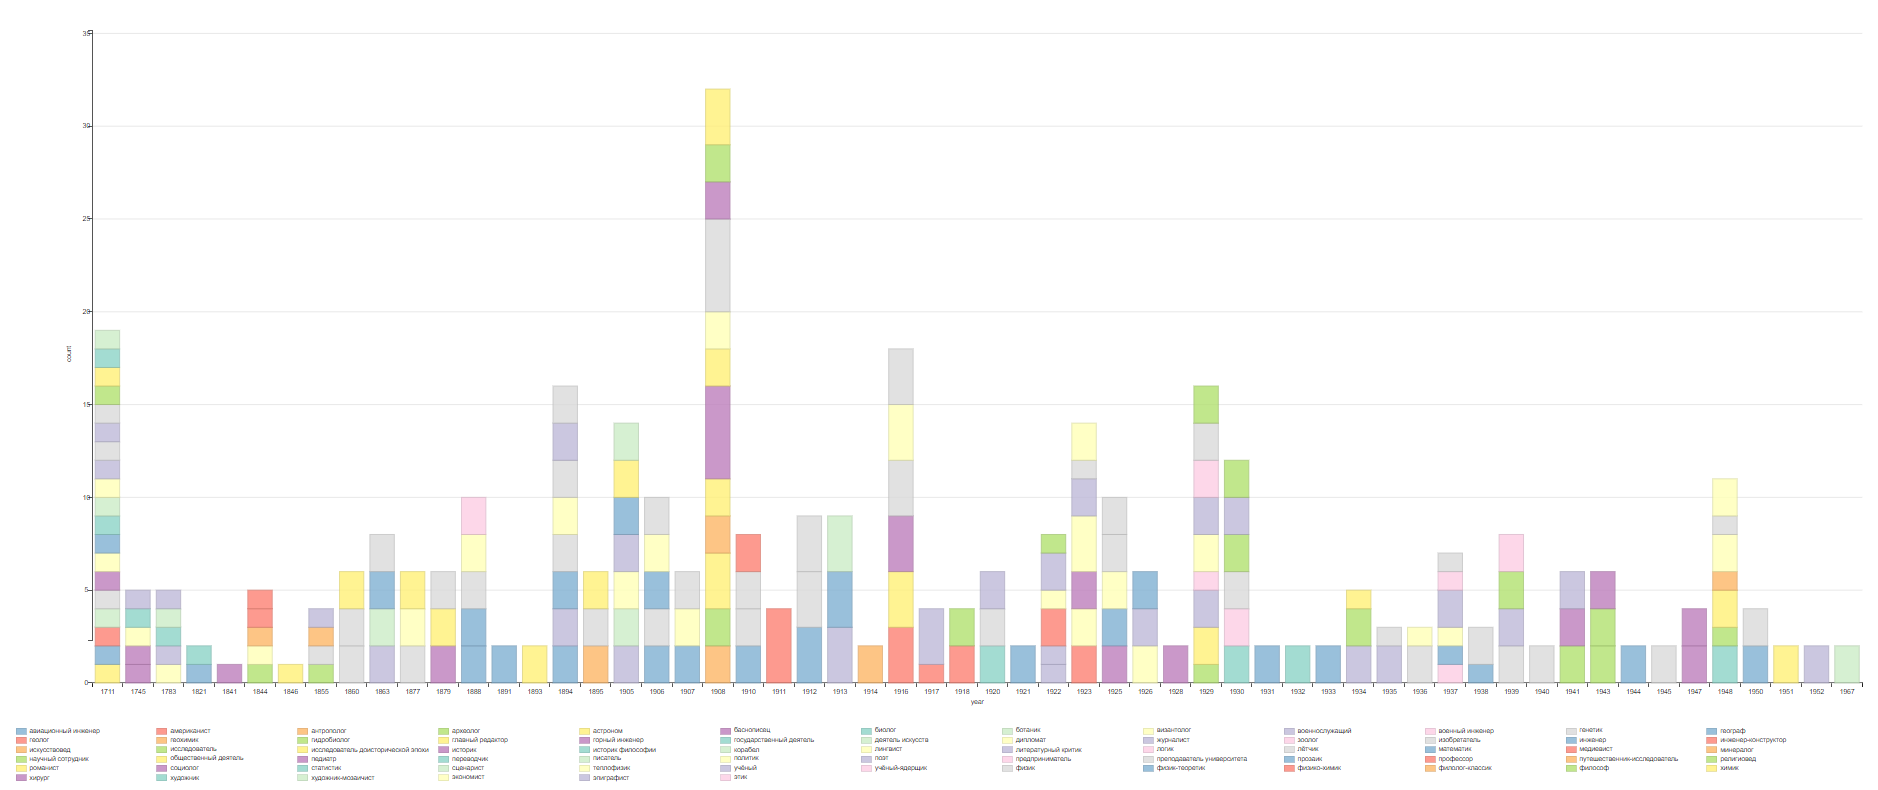
\includegraphics[width=1\linewidth]{./chapter/human_settlement/RussianScientistBornVillage.png}}
	\label{fig:human-settlement-5}
	\caption[Диаграмма количества ученых по родам деятельности родившихся в сельских полесениях.]{Диаграмма количества ученых по родам деятельности родившихся в сельских полесениях. Ссылка на SPARQL-запрос: \href{}{Длинная ссылка}.}%
\end{figure*} 

\begin{figure*}
    \setlength{\fboxsep}{0pt}%
    \setlength{\fboxrule}{1pt}%
    \fcolorbox{gray}{gray}{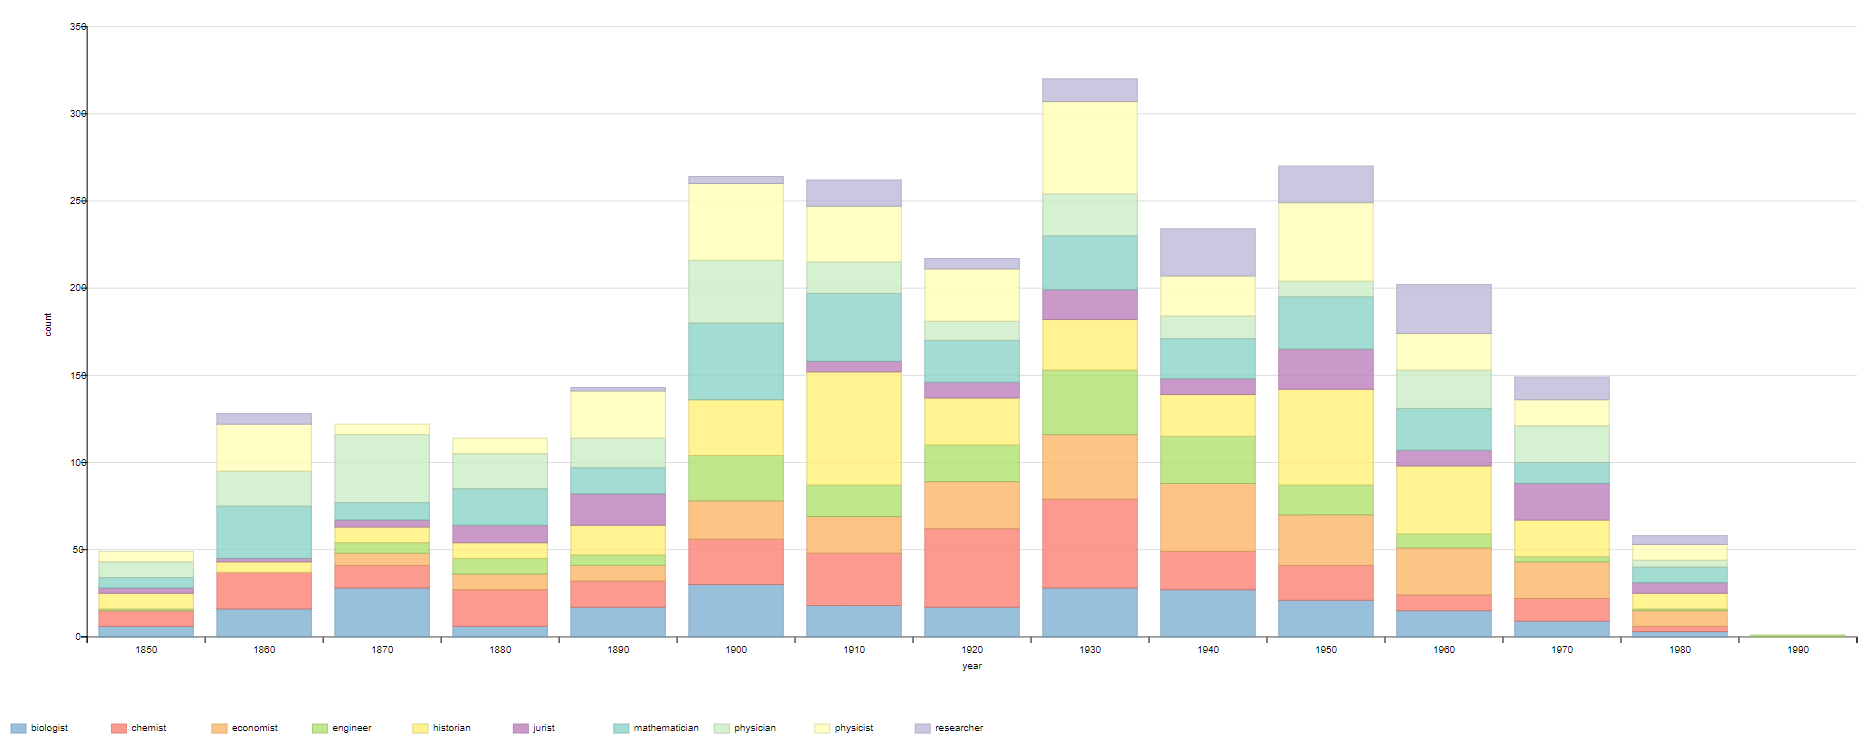
\includegraphics[width=1\linewidth]{./chapter/human_settlement/RussianScientistBornTown.png}}
	\label{fig:human-settlement-6}
	\caption[Диаграмма количества ученых по родам деятельности родившихся в городских полесениях.]{Диаграмма количества ученых по родам деятельности родившихся в городских полесениях. Ссылка на SPARQL-запрос: \href{}{Длинная ссылка}}%
\end{figure*} 
